\documentclass{MScthesisITEM}

% this package is just to generate text for demo-purposes
\usepackage{blindtext}


\title{Chip Power Estimation using GEM5} % The title of your assignement; NB use \newlinetitle to start a newline
\author{Terje Runde\newline Stian Hvatum} % Your firstname and lastname
\professor{Gunnar Tufte, IDI} % Affiliation = ITEM for instance
\supervisor{Gunnar Tufte, IDI}
\cosupervisor{Asbjørn Djupdal, IDI}

%% Uncomment the following in case you want subfigures; note that there will be a warning for the caption package
% \let\subcaption\undefined
% \let\subfloat\undefined
% \usepackage[bf]{caption}
% \usepackage{subcaption}

\DeclareGraphicsExtensions{.pdf,.jpg}
\graphicspath{{./figs/}}

\loadglsentries{glossary}
\makeglossaries

\begin{document}
\selectlanguage{english}
\pagenumbering{roman}
\pagestyle{plain}

%% Only for the project
\titleITEM

%% Only for the master's thesis; for the project report the description is taken from It's Learning and added by the department
% \selectlanguage{english} % Change to 'norsk' if you are writing in Norwegian
% \begin{titlingpage}

\noindent
\begin{tabular}{@{}p{4cm}l}
\textbf{Title:} 	& \thetitle \\
\textbf{Student:}	& \theauthor \\
\end{tabular}

\vspace{4ex}
\noindent\textbf{Problem description:}
\vspace{2ex}

\noindent \Blindtext[2][1]
\vspace{6ex}

\noindent
\begin{tabular}{@{}p{4cm}l}
\textbf{Responsible professor:} 	& \theprofessor \\
\textbf{Supervisor:}			& \thesupervisor \\
\end{tabular}

\end{titlingpage}
% \cleardoublepage

%% There must be an abstract in English, even though the main text is in Norwegian
\selectlanguage{english}
\pagestyle{empty}
\begin{abstract}

\noindent
    * dark silicon \\
    * power wall \\
    * shmac \\
    * good modelling tools \\
    * need for SIMPLE and EARLY STAGE energy estimations \\

    \noindent Since the beginning of semiconductor technology, transistor size has decreased and are still decreasing with a tremendous rate.
This has enabled engineers to build faster and faster single core processors. Faster and more dense processors 

, as there is more space for fancy solutions, and smaller
transistors means shorter switching latencies. In the last couple of years, processors have been kept down by the power wall, which
means that no more power can be dissipated without very clever cooling solutions. This turns out as a lot of space left for transistors
that we cannot use, a phenomenon called dark silicon.






The SHMAC project at NTNU aims to create a heterogeneous computer system that
can make use of dark silicon as space for energy efficient processors and special accelerators. Even though 













\end{abstract}

\cleardoublepage

%% Only for the master's thesis; if the main text is in English and you can write Norwegian, there must be an abstract in Norwegian as well.A
 \selectlanguage{norsk}
 \pagestyle{empty}
\renewcommand{\abstractname}{Sammendrag}
\begin{abstract}

    \noindent Energieffektivitet er en av de største utfordringene i moderne
    datamaskindesign. Videre ytelsesøkning begrenses av høy strømtetthet, i
    tillegg har energieffektivitet stor betydning i alt fra strømregningen på
    superdatamaskiner til batterlevetid for små innebygde enheter. Bedre
    forståelse for energieffektivitet vil gjøre det lettere å utvikle bedre
    arkitekturer. I denne masteroppgaven ser vi nærmere på arkitekturen og
    energiforbruket til en ARM Cortex-A9. Vi lager deretter et verktøy for å
    forutsi dens strømforbruk gjennom simulering.

    Gjennom målinger og eksperimenter gjort på ekte maskinvare bestemmes
    strømforbruk på instruksjonsnivå. Videre blir dette koblet til bestemte
    hendelser i den samme arkitekturen modelert i gem5-simulatoren. Verktøyet
    vårt benytter så disse hendelsene, sammen med loggfiler fra simulatoren, til
    å lage en representasjon av prosessorens strømforbruk over tid.

    Vår metode kan benyttes i prosessorutvikling allerede i simulatorfasen, mens
    tradisjonelle metoder ikke virker før maskinvaren er ferdig syntetisert.
    Resultatene viser at verktøyet vårt kan estimere strømforbruk innenfor 5~\%
    feilmargin på normale arbeidslaster. Det kan også identifisere positive og
    negative utviklinger i strømforbruket gjennom kjøringen av et program.

\end{abstract}

 \cleardoublepage

\selectlanguage{english}% Change to 'norsk' if you are writing in Norwegian

\renewcommand{\abstractname}{Preface}
\begin{abstract}
\noindent Think we need to figure out what this page should say...
\end{abstract}

\cleardoublepage

\begin{titlingpage}

\noindent
\begin{tabular}{@{}p{4cm}l}
\textbf{Title:} 	& \thetitle \\
\textbf{Student:}	& \theauthor \\
\end{tabular}

\vspace{4ex}
\noindent\textbf{Problem description:}
\vspace{2ex}

\noindent \Blindtext[2][1]
\vspace{6ex}

\noindent
\begin{tabular}{@{}p{4cm}l}
\textbf{Responsible professor:} 	& \theprofessor \\
\textbf{Supervisor:}			& \thesupervisor \\
\end{tabular}

\end{titlingpage}
\cleardoublepage
% similarly you may add a separate acknowledgments page

\tableofcontents*
\cleardoublepage

%% include if relevant
\listoffigures
\cleardoublepage

%% include if relevant
\listoftables
\cleardoublepage

%% include if relevant
\listofalgorithms
\addcontentsline{toc}{chapter}{List of Algorithms}
\cleardoublepage

%% include if relevant
\printglossary[title=List of Symbols, style=long]
\cleardoublepage
\glsaddall[]

%% include if relevant
\printglossary[title=List of Acronyms,type=\acronymtype] % prints just the list of acronyms
\cleardoublepage

\pagenumbering{arabic}
\pagestyle{ruled}
\chapter{Introduction}

\chapter{Background}

This thesis touches subjects crossing both  artificial intelligence, computer
architecture and electronics. Some background information on the  most important subjects are
provided in this chapter.

\section{CPU-level Energy Measurements}

High quality instruction level energy models can be derived for pipelined
processors by monitoring the instantaneous current drawn by the processor at
each clock cycle \cite{nikolaidis2005instruction}. Modern processors commonly
operate at a few GHz, which means that expensive measurement devices are
required to sample at sufficient frequency. According to Harry Nyquist the
sampling frequency must be twice the speed of the signal being measured
\cite{nyquist1928certain}. As the signal sampled from the processor might
change at least once every clock tick, a cycle accurate measurement would
require the instrumentations would have to sample much faster than any equipment
available at our laboratory.

In \cite{rundehvatum2013exploring}, single instructions was measured by
exploting fast-loop-mode and looping over a group of equal instructions. An
Agilent bench multimeter and a shunt resistor was set up like shown in
\autoref{fig:setup}.  This method provides an average power consumption when the
pipeline is (mostly) filled with a single type of instruction. Instead of normal
serial connected ammeter, the power rail is connected in series with a shunt
resistor equal to the one display in \autoref{fig:shunt}, and the almost
neglectable voltage drop over this resistor is measured using a voltmeter. This
method provides a way to measure currents outside the range of the ammeter.

\begin{figure}
    \centering
    \input{figs/test_setup.tex}
    \caption{Bench setup for measuring single instruction current drain}
    \label{fig:setup}
\end{figure}

\begin{figure}
    \centering
    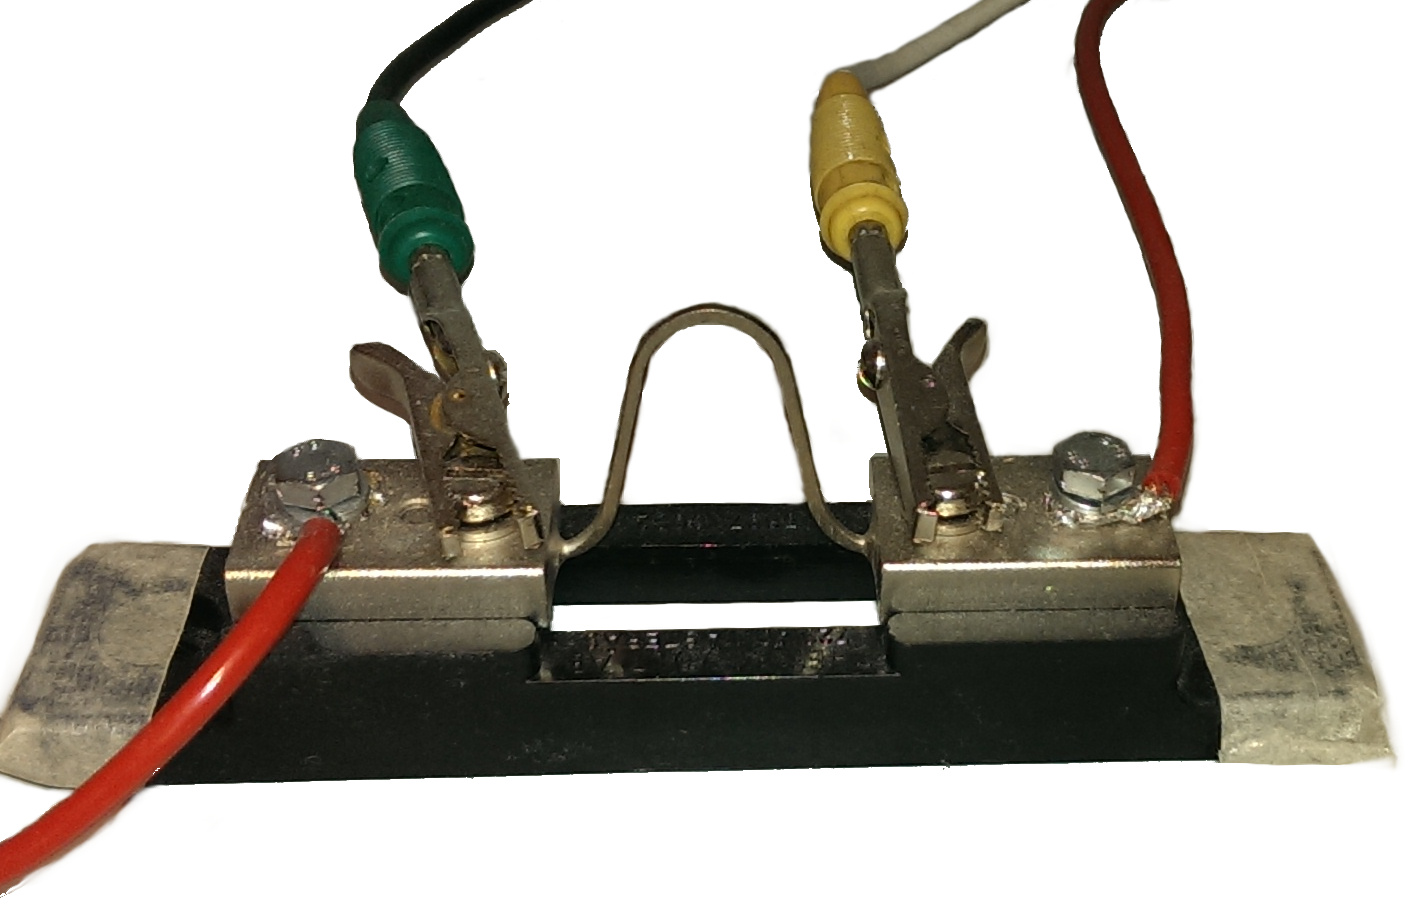
\includegraphics[width=0.8\textwidth]{figs/shunt.jpg}
    \caption{An example shunt resistor}
    \label{fig:shunt}
\end{figure}

% TODO: Where does this fit?
% The ultimate goal in this context is to estimate power consumption and energy
% efficiency of new hardware, the first step is to measure different more or less
% power consuming events on real hardware that is similar to the one simulated.


\section{Hardware Platform}

The ODROID-X2 developer platform \cite{hardkernelodroidx2} is used as a
reference hardware for all experiments in this thesis. An image of the platform
is shown in \autoref{fig:odroidx2}. Its core voltage is easily accessible on an
attached daughter board right beneath the heat sink, making it easy to conduct
power measurements. The board is equipped with a Samsung Exynos 4412 ``Prime'',
a modern System-on-Chip featuring four ARM Cortex-A9 CPU cores, Mali-400 GPU and
2~GB of on-chip DRAM. The Cortex-A9 is one of ARM's mid-to-high-range application
processors. It features an out-of-order dual-issue speculative RISC core, and it
is clearly designed with emphasis on energy efficiency. This processor is
primarily found in low-powered embedded devices with some performance demands,
typically smartphones and tablets.

\begin{figure}[bth]
    \centering
    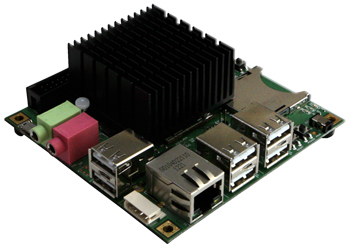
\includegraphics[width=0.7\textwidth]{figs/odroid.jpg}
    \caption{Image of the Hardkernel ODROID-X2 from the Hardkernel ODROID-X2 product page \cite{hardkernelodroidx2}}
    \label{fig:odroidx2}
\end{figure}

\begin{table}
    \centering
    \begin{tabular}{|c|c|}
        \hline
        Component      & Spesification\\
        \hline
        Manufacturer   & Hardkernel \\
        Platform       & ODROID-X2 \\
        SoC            & Samsung Exynos 4412 ``Prime'' \\
        CPU Core       & ARM Cortex-A9 \\
        Number of Cores& 4 \\
        Clock Frequency& 1.7~GHz \\
        Core Voltage   & 1.3~V \\
        L1             & Dual 32~KB \\
        L2             & 1~MB \\
        Main memory    & 2~GB LP-DDR2 880~MHz \\
        \hline
    \end{tabular}
    \caption{Hardware specifications ODROID-X2}
    \label{tab:hwspecx2}
\end{table}

As seen in \autoref{fig:a9arch} there is an out-of-order multi-issue module
right after the decode stage. This module can do speculative issue and can
schedule two arithmetic operations, in which one can be a multiply (the
processor has only one hardware multiply unit). It also features a multiplexed
lane for address operations and floating point operations (the \emph{NEON} FPU).
In this experiment, a 4-core variant of the processor was used, but 3 of the
cores was disabled to ease both the measurement and the simulation process.

\begin{figure}[bht]
    \centering
    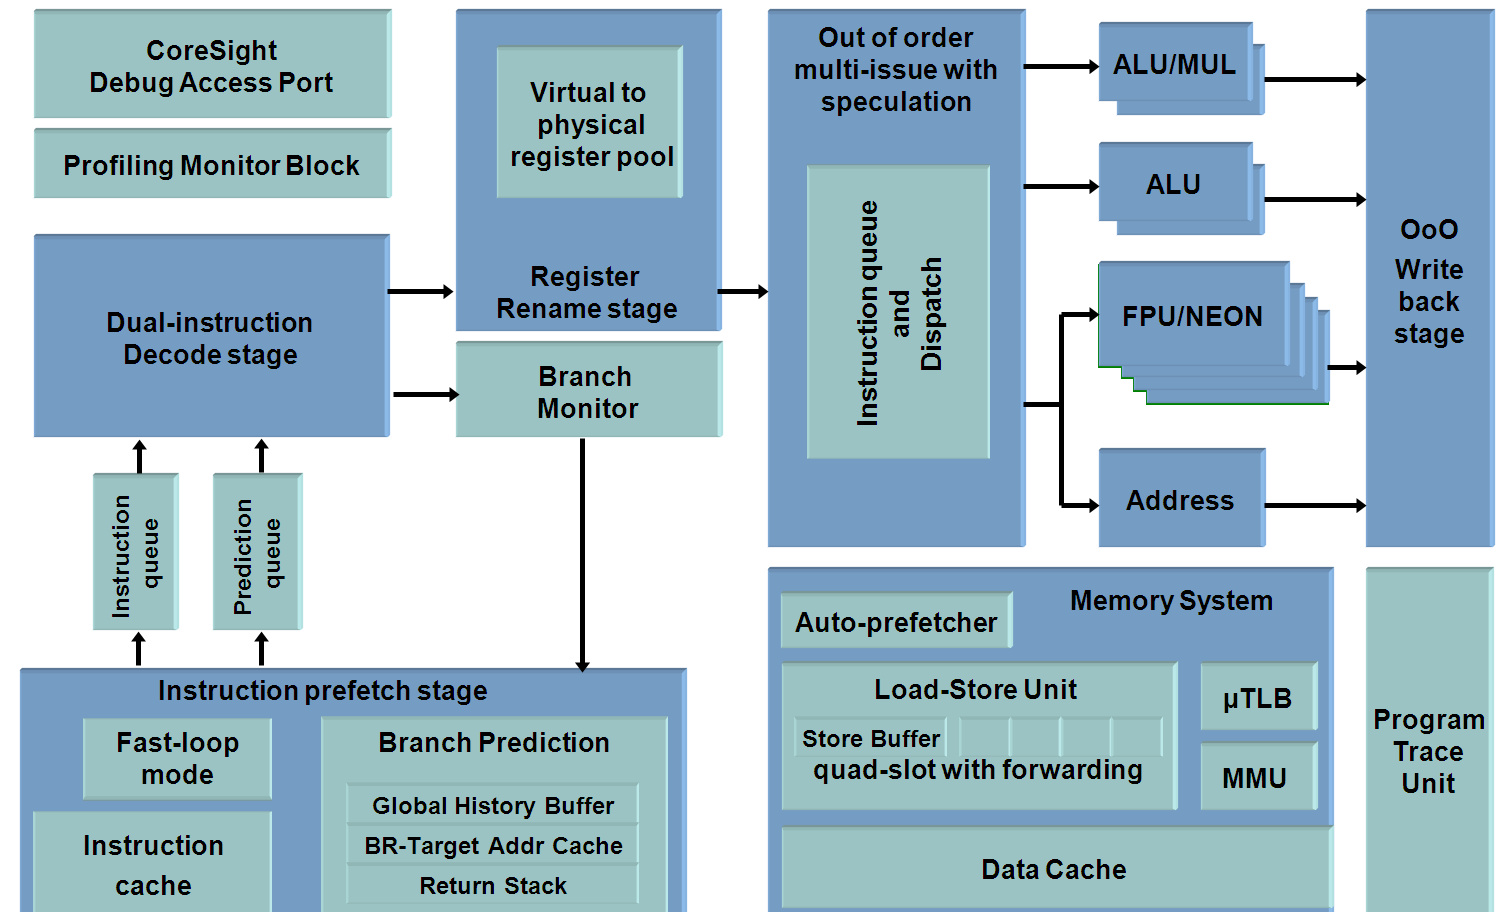
\includegraphics[width=0.8\textwidth]{figs/A9-Pipeline-hres.jpg}
    \caption{A brief overview of the Cortex A9 Pipeline, figure from the ARM Cortex-A9 Whitepaper \cite{a9whitepaper}}
    \label{fig:a9arch}
\end{figure}

To achieve good simulation correctness, a high level of architectural knowledge
is crucial. Despite that most proprietary architectures have a lot of details
that remain undisclosed to the public, much information is still available.
Different sources have been used to find properties needed by the simulator,
some details regarding the OoO cores can be read about in
\cite{blem2013detailed}.

\section{Hardware Simulators}

As computer architecture development meets more challenging demands, a versatile
set of software tools have been developed to help the designers. In this set of
tools lies a set of computer architecture simulators meant to evaluate
processors at the architectural level. The simulators often provides the ability
to write hardware in a language more abstract than HDL-languages, provides the
ability to run compiled binaries, and provides detailed trace logs and
performance data. The benefits of architectural simulators are many, but it is
important to find one that fits the demands given by the problem.

\subsection{A Brief Comparison}
\label{subsec:simulators}
There are numerous computer architecture simulators available to the public,
both commercial, free and open source alternatives exists. To support our power
estimation tool, a simulator frontend must provide a good picture of events
that occur in a hardware implementation of the architecture. The hardware
platform used for reference in this thesis is an out-of-order ARM Cortex-A9
based core fitted with memory and and peripherals in a von Neumann architectural
scheme. The out-of-order property significantly increases the level of
complexity which the simulator must handle.

\begin{description}
\item[Sniper] \hfill\\
    Sniper is a high-speed, multicore, multi-threaded and cycle-accurate
    computer architecture simulator \cite{sniperwebpage,carlson2013ssomta}. It
    already integrates with McPAT and it is open source. Sniper does only work
    x86, and is thus not applicable for simulation of ARM-based architectures.

\item[SimpleScalar] \hfill\\
    SimpleScalar is a popular commercial architectural simulator that comes with
    a free academic license providing full source code. SimpleScalar supports
    the ARM instruction set amongst many others, and looks like a decent
    simulator for advanced out-of-order core simulation. SimpleScalar is also
    the simulator used by the Wattch-project \cite{brooks2000wattch}. However,
    the SimpleScalar web page seems to be last updated in 2004 and all mailing
    list archives are gone at the time of writing. The source code for
    SimpleScalar v3 is still available, but has only been patched once since
    2003.

\item[QEMU]\hfill\\
    QEMU is a generic and open machine emulator which enables near real-time
    performance on architectures like ARM, even on x86 host machines. However,
    QEMU is a machine emulator rather than an architectural simulator, thus
    despite its great performance of running ARM-binaries, it will not produce
    CPU and memory event trace logs, and is not suitable for this project.

\item[gem5]\hfill\\
    gem5 is a merger between the M5 simulator \cite{binkert2006m5} and the GEMS
    simulator project \cite{GEMS}. gem5 provides ARM-support with out-of-order
    execution out of the box, and provide great cycle-accurate trace logs which
    are appropriate for this project \cite{gem5simulator}. Its core is written
    in C++ and has a highly modular interface that allows users to specify
    simulator target through simple Python scripts. Many of the maintainers are
    employees of ARM Corp., and the activity on the mailing lists suggests high
    project activity \cite{gem5dev}.
\end{description}

Provided this comparison of simulators, and given the fact that NTNU has a tradition
for using M5 and gem5 in earlier research projects and subjects, gem5 is the natural
winner for the choise of an architectural simulator.


\subsection{The gem5 Simulator}

The gem5 project \cite{gem5} merges the best features of M5 \cite{binkert2006m5}
and GEMS \cite{GEMS} and includes a wide range of CPU and memory models
\cite{gem5hipeac}. The simulator has two main execution modes; \textit{Syscall
Emulation} (SE) or \textit{Full System} (FS). In SE mode, the simulator traps
system calls in the binary and emulates them, often by passing them to the host
operating system. In FS mode, the simulator can load an operating system binary
and run application within the OS. The latter mode is well suited when the OS in
its entirety must be simulated. gem5 supports many architectures; it can run
binaries compiled for ALPHA, SPARC, MIPS, ARM, x86 and POWER architectures.

During simulation, gem5 keeps track of hundreds of events related to the CPU
core and memory system. In-detail statistics, similar to performance counters on
real hardware, are then dumped for subsequent inspection. gem5 is also able to
output a trace log while it runs, originally intended for debugging of gem5.A
trace log contains user-selected events that happens within the simulated
hardware. These trace logs grow quickly in size, easily 10s of gigabytes, but
provides useful insights of the simulated execution. In particular, they describes
CPU activity down to the microarchitecture level and outputs simulated processor
activity.


\section{Parameter Optimization}


\subsection{Genetic Algorithms}

\section{SHMAC}

SHMAC is a hardware prototype of a Single-ISA Heterogeneous MAny-core Computer
\cite{shmacsliedes, shmacwebpage, Rusten567042}. It is an ongoing research
project within the Energy Efficient Computing Systems (EECS) research area at
the Department of Computer and Information Science at NTNU. The SHMAC project is
driven by the \textit{dark silicon effect}; as transistors become smaller, only
parts of a chip can be powered simulataneously \cite{esmaeilzadeh2011dark}.
SHMAC implements two main strategies to mitigate the dark silicon effect,
heterogeneity and specialization.

\begin{figure}
    \centering
    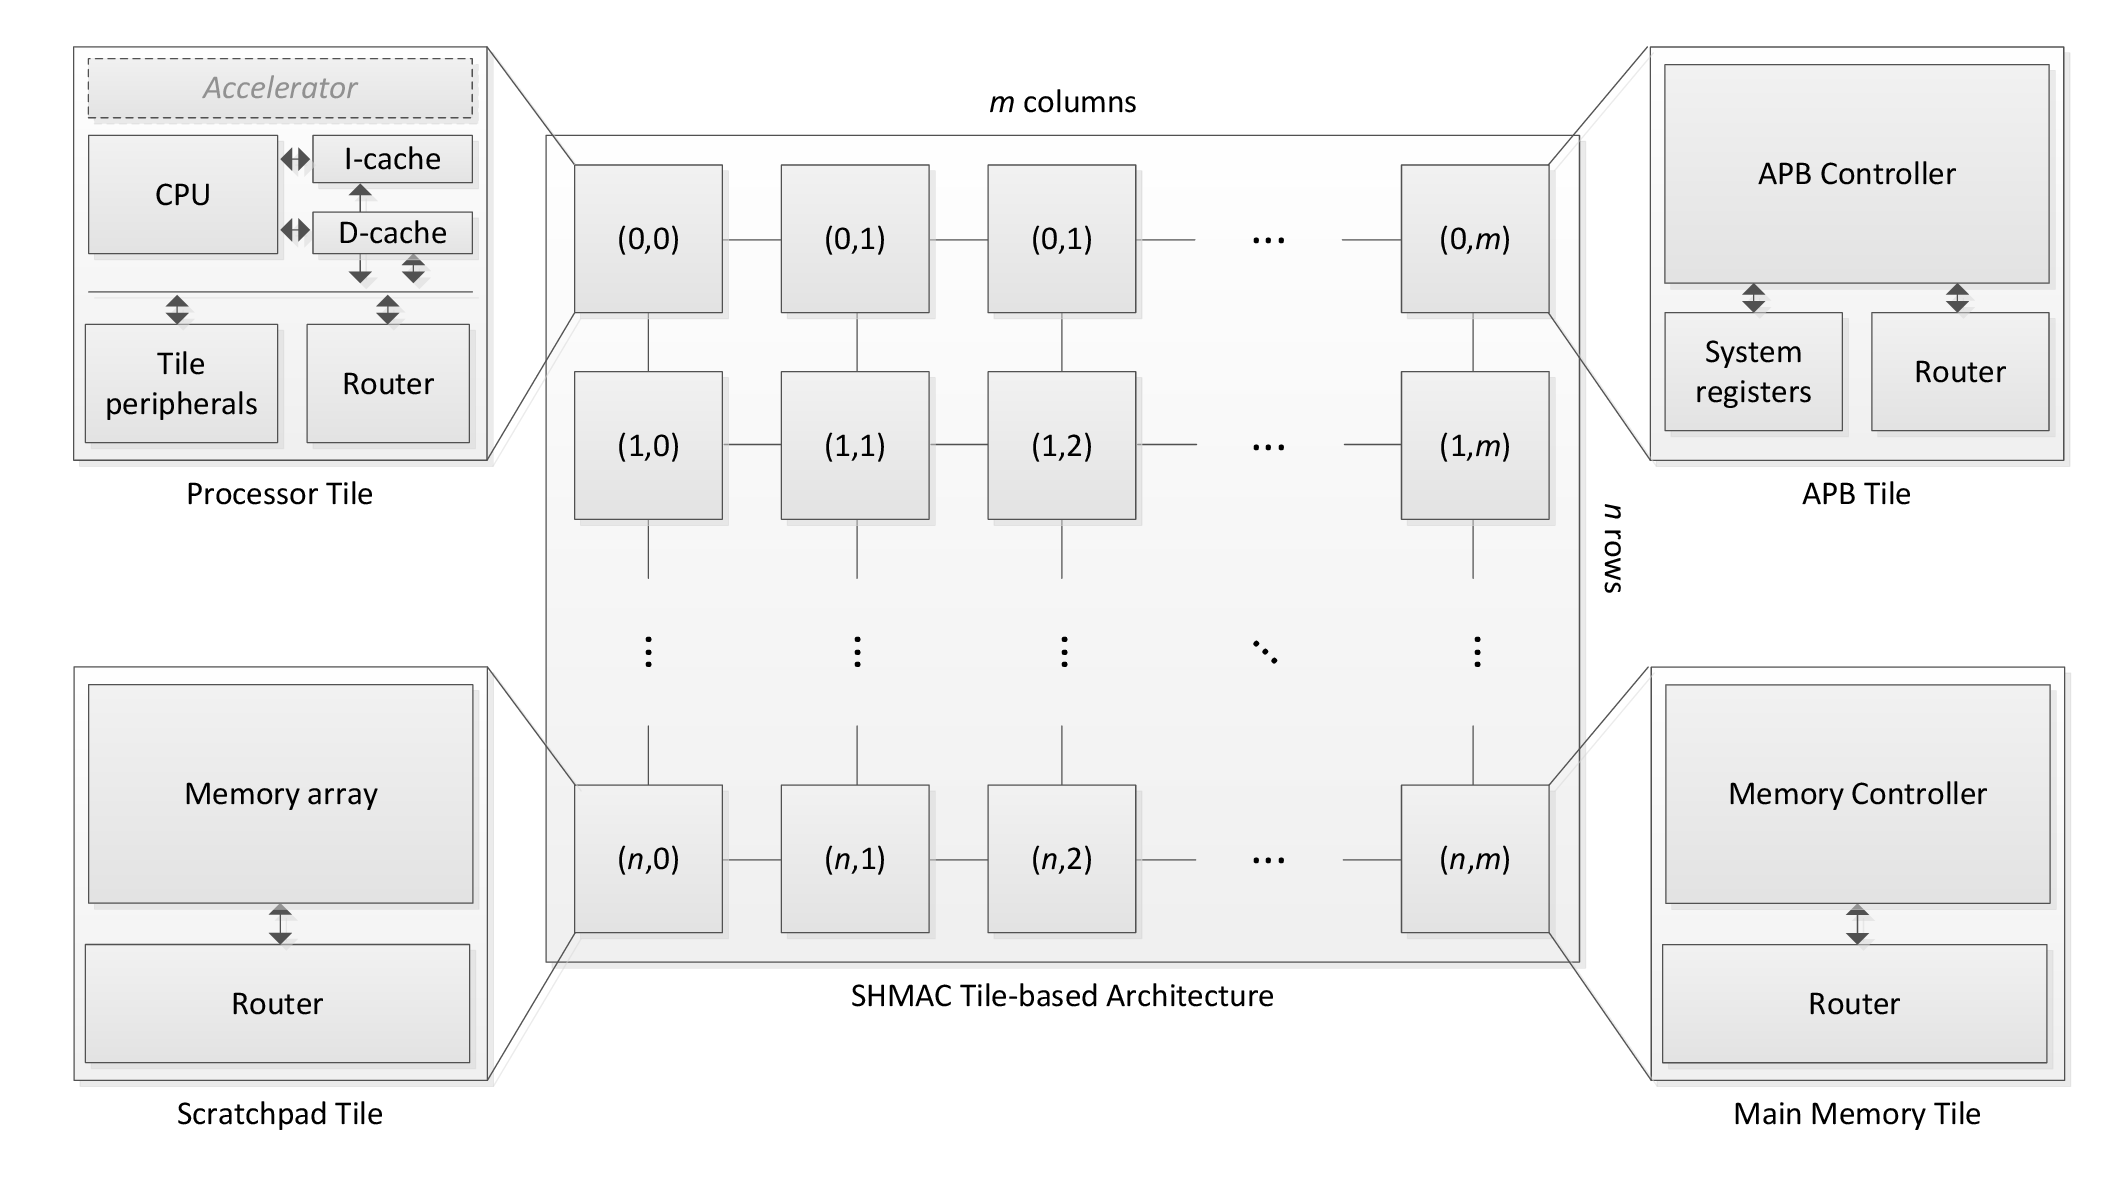
\includegraphics[width=1.0\textwidth]{figs/shmac-high-level2.png}
    \caption{}
    \label{fig:shmac}
\end{figure}

The SHMAC architecture is tile-based. Processing elements are laid out in a
rectangular grid with connections to their nearest neighbor, as depicted in
\autoref{fig:shmac}. A router protocol present in all SHMAC tiles handles
communication and data flow between tiles.  The great deal about SHMAC is that
different kinds of specialized tiles/accelerators can be composed as desired, to
form a computer tailored to the application.


\chapter{Example}
\label{chp:example} 

Here is an example of how to use acronyms such as \gls{ntnu}. The second time only \gls{ntnu} is shown and if there were several you would write \glspl{ntnu}. And here is an example\footnote{A footnote} of citation~\cite{Author:year:XYZ}. 

\Blindtext[3][1]

\begin{figure}
\centering
% dummy figure replacement 
\begin{tabular}{@{}c@{}}
\rule{.5\textwidth}{.5\textwidth} \\
\end{tabular}
\caption{\label{fig:example}A figure}
\end{figure}

\section{First section}\label{sec:first_section}

\subsection{First subsection with some \texorpdfstring{$\mathcal{M}ath$}{Math} symbol}\label{sec:first_ssection}

\blindtext
\begin{itemize}[topsep=-1em,parsep=0em,itemsep=0em] % see http://mirror.ctan.org/macros/latex/contrib/enumitem/enumitem.pdf for details about the parameters
 \item item1
 \item item2
 \item ...
\end{itemize}

\subsection{Mathematics}

\blindmathtrue
\blindtext

\begin{proposition}\label{def:a_proposition}
A proposition... (similar environments include: theorem, corrolary, conjecture, lemma)

\end{proposition}

\begin{proof}
\vspace*{-1em} % Adjust the space when parskip is set to 1em
And its proof.
\end{proof}

\begin{table}
\caption{\label{tab:example}A table}
\centering
\begin{tabular}[b]{| c | c | c | c | c |}
\hline
a & b & c & d & e \\ \hline
f & g & h & i & j \\ \hline
k & l & m & n & o \\ \hline
p & q & r & s & t \\ \hline
u & v & w & x & y \\ \hline
z & æ & ø & å &   \\ \hline
\end{tabular} 
\end{table}

\subsection{Source code example}

% \floatname{algorithm}{Source code} % if you want to rename 'Algorithm' to 'Source code'
\begin{algorithm}[h]
  \caption{The Hello World! program in Java.}
  \label{hello_world}
  % alternatively you may use algorithmic, or lstlisting from the listings package
  \begin{verbatim}
  
class HelloWorldApp {
  public static void main(String[] args) {
    //Display the string
    System.out.println("Hello World!");
  }
}
\end{verbatim}
\end{algorithm}

You can refer to figures using the predefined command like \fref{fig:example}, to pages like \pref{fig:example}, to tables like \tref{tab:example}, to chapters like \Cref{chp:example} and to sections like \Sref{sec:first_section} and you may define similar commands to refer to proposition, algorithms etc.

%% include here the other chapters

\renewcommand*{\bibname}{References}
\bibliographystyle{alpha}
\bibliography{main}

%% Uncomment the following if you have any appendix
% \appendix
% \addtocontents{toc}{%
%  \protect\vspace{1em}% 
%  \protect\noindent \bfseries \appendixtocname\protect\par
%  \protect\vspace{-.5em}%
% }
% \renewcommand{\chaptername}{\appendixname}
%% include below possible appendices (chapters)


\end{document} 
